\chapter{Introduction}
\label{sec:introduction}
%\chapter{Einleitung}
%\label{sec:einleitung}

One of the key challenges on the way towards autonomous robot navigation is localization. To achieve any autonomous task, a robot needs to estimate its pose, which is the robot's position and orientation in space. Visual-inertial Localization is one approach to estimate the robot's pose by combining the information of an inertial measurement unit (IMU) and the information retrieved by a camera. A camera image provides rich structure information about the scenery and IMU measurements help estimating the robot's pose over short distances. Due to these complementary properties a camera-IMU sensor system is well suited for the complex task of robot localization. The visual-inertial approach has some key advantages in comparison to approaches using other information sources like laser range finders or external localization systems: camera and IMU are lightweight sensors, which can be equipped on a flying robot; they are passive sensors with a small energy consumption; and they are onboard sensors, which can be applied in GPS-denied environments without modifying the environment itself. \\


\begin{figure}[h]
   \centering
   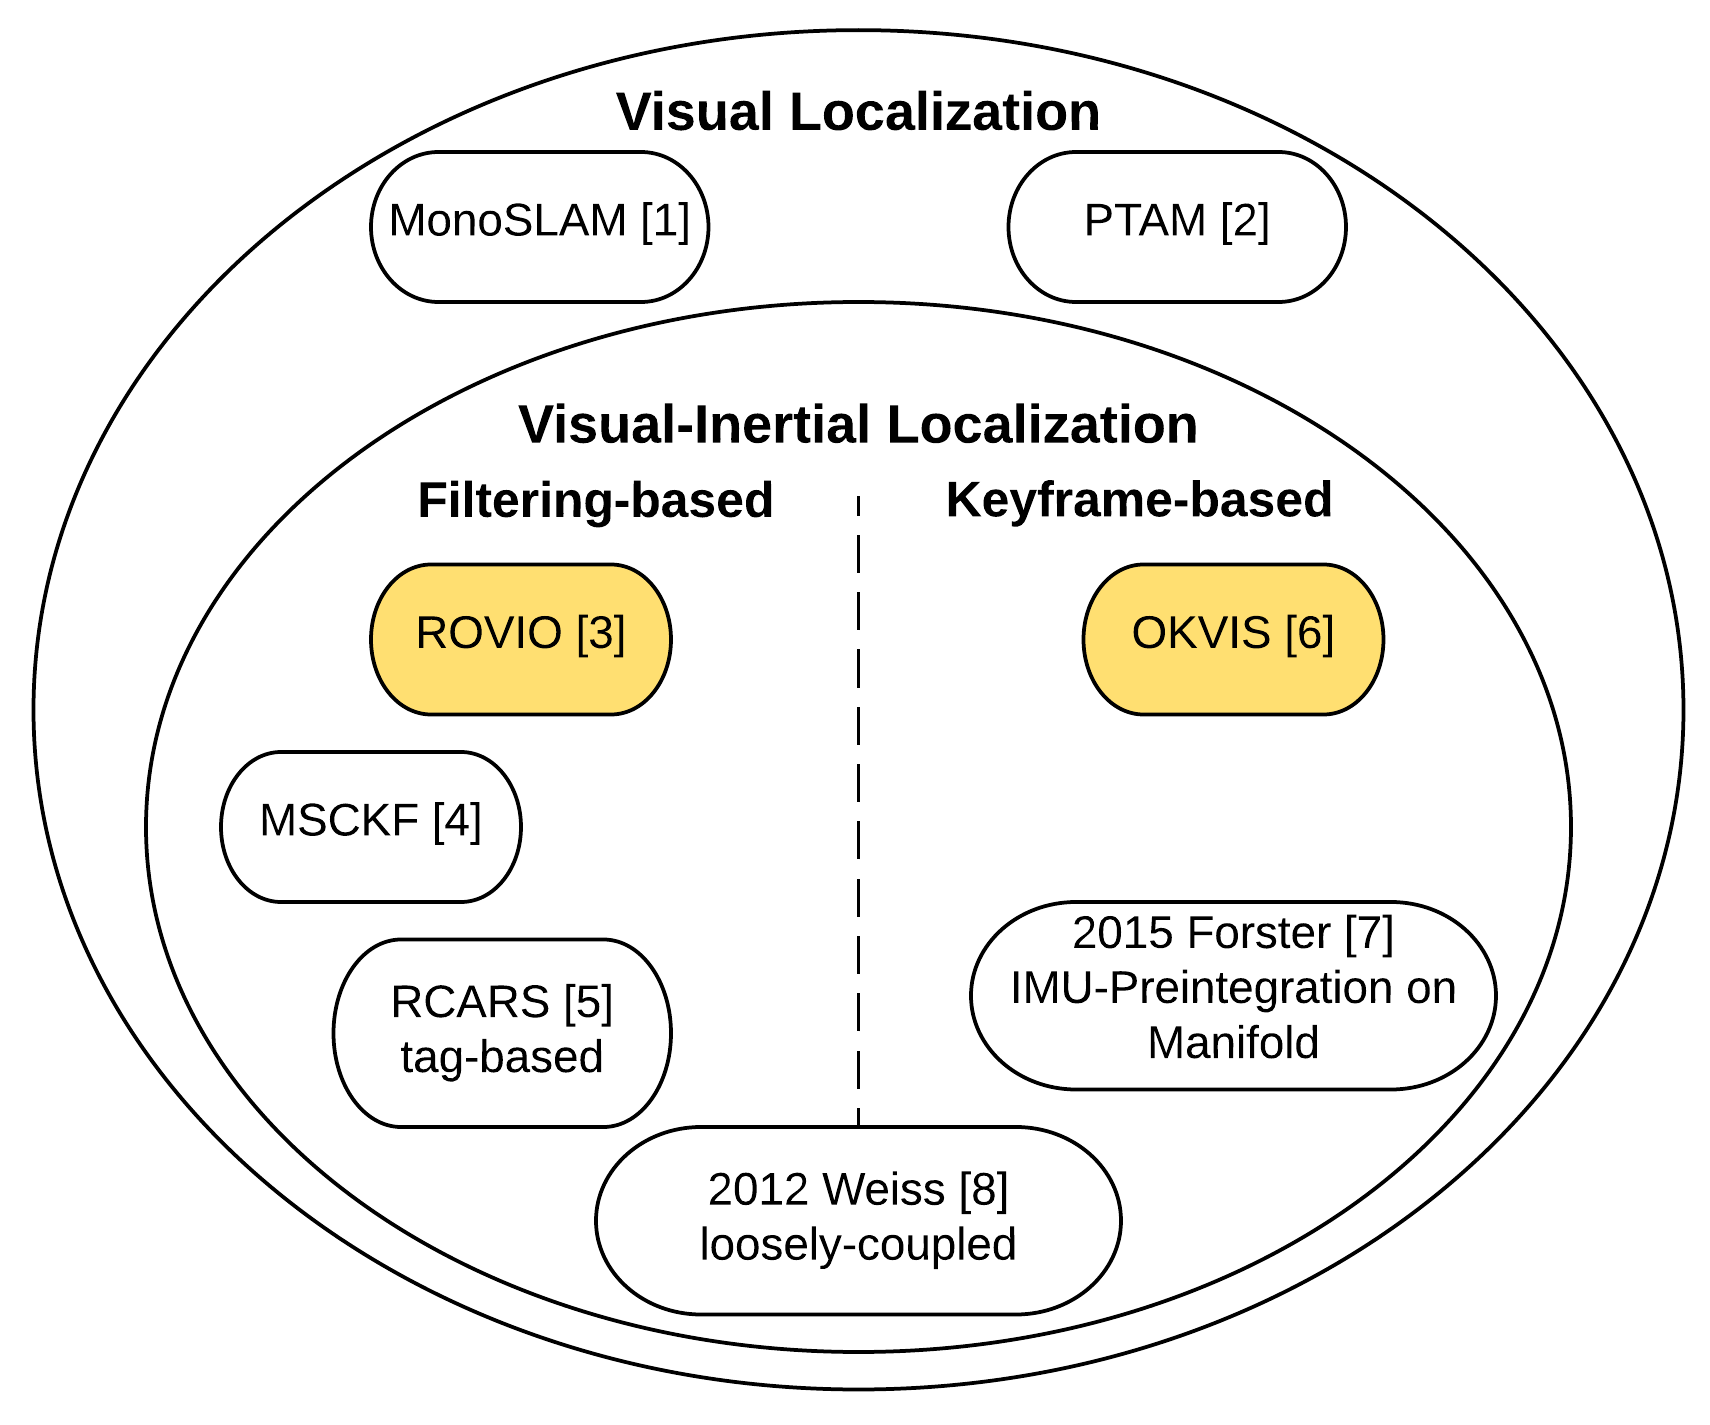
\includegraphics[width=0.6\textwidth]{images/state_of_the_art.png}
   \caption{State of the art for the field of visual localization and for the visual-inertial localization in particular.}
   \label{pics:state_of_the_art}
\end{figure}
% SVO \cite{forster2014svo}
% LSD-SLAM \cite{engel2014lsd}

Over the last decade, a series of different algorithms achieving visual-inertial robot localization have been proposed. Figure \ref{pics:state_of_the_art} shows an overview of the field of visual localization and that of visual-inertial localization in particular. Considerable work has been achieved with MonoSLAM (Davison et al. \cite{davison2007monoslam}), who introduced a framework for simultaneous localization and mapping (SLAM) based on a single camera that is running in real-time, and PTAM, Parallel Tracking and Mapping (Klein et al., \cite{klein2007parallel}), who achieved an enhancement regarding computational complexity by parallelizing the mapping and tracking functionalities into two separate threads. \\

Visual-inertial localization can be divided into the inherently different filtering-based and keyframe-based approaches. 

The filtering-based approach (figure \ref{pics:filtering_keyframe} a) achieves robot localization by propagation of the estimated pose based on the IMU measurements and updating this prior belief based on the camera observation. In the filtering-based approach, an estimate of the state in the past will never be corrected based on a new observation. Because of this property, filtering-based algorithms are more prone to drift, but computationally less expensive than the keyframe-based implementations. ROVIO, robust visual-inertial odometry (Blösch et al., \cite{bloeschrobust}) is a recent and promising implementation of the filtering-based approach using an extended kalman filter (EKF) and direct intensity image patches. Other promising filtering-based algorithms include MSCKF, a multi-state constraint kalman filter (Mourikis et al., \cite{mourikis2007multi}), who introduced a filter working on the information of a set of past frames and RCARS, robot-centric absolute reference system (Neunert et al., \cite{neunert2015open}), who demonstrated a filtering-based localization system for a scenery with artificial tags included.

The keyframe-based approach (figure \ref{pics:filtering_keyframe} b) achieves robot localization by a nonlinear optimization. OKVIS, optimal keyframe-based visual inertial SLAM (Leutenegger et al., \cite{leutenegger2015keyframe}) is one promising implementation of this approach, which includes both, the camera and IMU information into a single error function. Another recently published and promising keyframe-based implementation applies a direct approach with preintegration of the IMU measurements (Forster et al., \cite{forster2015imu}).

In addition to the filtering-based and keyframe-based approach, an implementation has been proposed that combines the two approaches in a loosely-coupled way, by performing a keyframe-based implementation on the vision side and fusing the result afterwards in a filter with the IMU information (Weiss et al., \cite{weiss2012real}). \\

\begin{figure}
  \begin{subfigure}[b]{0.4\textwidth}
    \captionsetup{skip=6pt}
    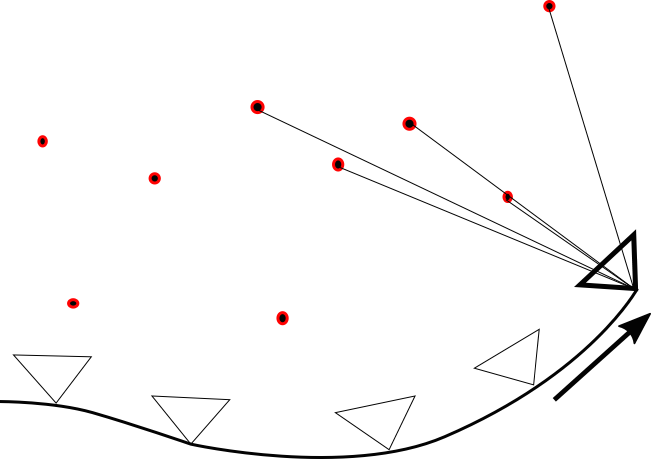
\includegraphics[width=\textwidth]{images/filteringbased_2.png}
    \caption{filtering-based}
    \label{fig:1}
  \end{subfigure}
  \hfill
  \begin{subfigure}[b]{0.4\textwidth}
    \captionsetup{skip=6pt}
    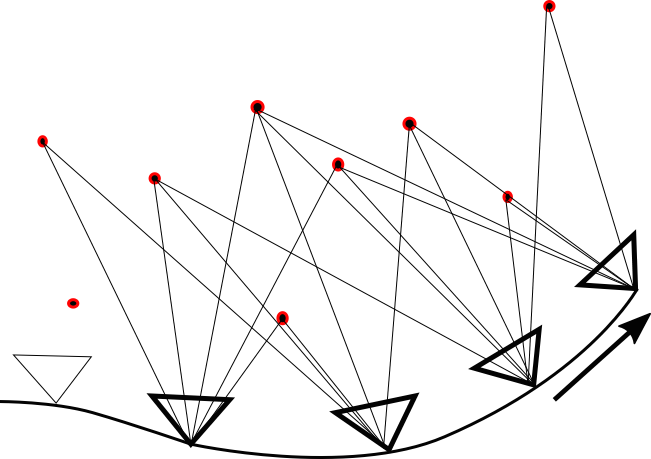
\includegraphics[width=\textwidth]{images/keyframebased_2.png}
    \caption{keyframe-based}
    \label{fig:2}
  \end{subfigure}
\caption{(a) shows the filtering-based principle of localization: the robot's pose is propagated between two camera frames based on the IMU measurements and updated based on the cameras landmark observations. The pose of a past frame is not corrected based on a new observation. (b) shows the keyframe-based approach to localization: the robot's pose is estimated by a nonlinear optimization based on the IMU data and the landmark observations of a \textit{set} of frames. With this approach the pose of a past frame is corrected based on a new observation.}
\label{pics:filtering_keyframe}
\end{figure}

Strasdat et al., \cite{strasdat2010real}, showed, that the keyframe-based approach is preferable to the filtering-based approach whenever the computational resources are available. But, the ongoing research in both domains, the superior performance of the filtering-based approach regarding computational complexity, and the robustness of filtering-based implementations, demonstrate the significance of both approaches until today. \\

This work presents a direct comparison of the filtering-based algorithm ROVIO and the keyframe-based algorithm OKVIS on real data. Both algorithms show promising results, have been developed at ETH Zurich and are on the way of being published open source. As all state of the art algorithms, OKVIS and ROVIO show drift issues. These drift issues will be analysed and quantified. 

On the way towards a generic visual-inertial localization, the robustness of an algorithm with respect to different sensor systems is of importance. So far, ROVIO and OKVIS have only be proven to run on a hardware-wise time synchronized sensor system. Within the scope of this report, an experimental analysis is presented that approaches the question if ROVIO is able to work with a more generic, non time synchronized, sensor system. \\

The following sections \ref{sec:rovio} and \ref{sec:okvis} introduce the working principles and characteristics of ROVIO and OKVIS, respectively. Section \ref{sec:metrics} introduces the evaluation metrics and presents a differentiation between global and local accuracy. The results and their discussion can be found in section \ref{sec:results}: \ref{sec:ijrr} contains the comparison between ROVIO and OKVIS based on indoor data collected with a hardware-wise time synchronized sensor system and section \ref{sec:euroc} gives some deeper insights into the ROVIO performance on a complementary dataset. The analysis whether ROVIO is able to work with a generic sensor system is presented in section \ref{sec:timesync}. \\
